\id{IRSTI 52.35.29}{}
\vspace{1.5em}
\begin{articleheader}
\sectionwithauthors{A.D. Shontayev, T.V. Demina, D.S. Shontaev, V.F. Demin, D.D. Meiram}{THE IMPORTANCE OF THE GAS FACTOR IN THE OCCURRENCE OF SUDDEN OUTBURST OF COAL AND GAS}

{\bfseries
\textsuperscript{1}A.D. Shontayev\alink{https://orcid.org/0000-0003-1411-508X;},
\textsuperscript{2}T.V. Demina\alink{https://orcid.org/0009-0006-1607-3097},
\textsuperscript{1}D.S. Shontaev\alink{https://orcid.org/0009-0003-5024-0838},
\textsuperscript{3}V.F. Demin\alink{https://orcid.org/0000-0002-1718-856X},
\textsuperscript{3}D.D. Meiram\alink{https://orcid.org/0009-0003-6092-4790}\textsuperscript{\envelope}
}
\end{articleheader}

\begin{affiliation}
\textsuperscript{1}Kulazhanov Kazakh University of Technology and Business, Astana, Kazakhstan,

\textsuperscript{2}Ural State Mining University, Ekaterinburg, Russian Federation,

\textsuperscript{3}Saginov Technical University, Karagandy, Kazakhstan.

\raggedright \textsuperscript{\envelope }Corresponding-author: \href{mailto:baiz76@mail.ru}{diana\_meiram@mail.ru}
\end{affiliation}

The article examines the role of methane contained in coal in the
mechanism of sudden outburst, because practice shows that the amount of
methane released per ton of coal released into mining is several times
and even tens of times higher than the natural gas content of the coal
seam. Establishing the causes of sudden outbursts is necessary to reduce
the risk of outbursts by influencing the stress state of a gas-saturated
coal seam.

{\bfseries Keywords:} sudden outburst of coal and gas, outburst hazard, gas
content, gas release, gas saturation.

\begin{articleheader}
{\bfseries КӨМІР МЕН ГАЗДЫҢ КЕНЕТТЕН ШЫҒАРЫЛУЫНЫҢ ПАЙДА БОЛУЫНДАҒЫ ГАЗ ФАКТОРЫНЫҢ МАҢЫЗЫ}

{\bfseries
\textsuperscript{1}А.Д. Шонтаев,
\textsuperscript{2}Т.В. Демина,
\textsuperscript{1}Д.С. Шонтаев,
\textsuperscript{3}В.Ф. Демин,
\textsuperscript{3}Д.Д. Мейрам\textsuperscript{\envelope }
}
\end{articleheader}

\begin{affiliation}
\textsuperscript{1}Құлажанов атындағы Қазақ технология және бизнес университеті, Астана, Қазақстан,

\textsuperscript{2}Орал мемлекеттік тау-кен университеті, Екатеринбург, Ресей Федерациясы,

\textsuperscript{3}Сағынов атындағы Қарағанды техникалық университеті, Қарағанды, Қазақстан,

e-mail: \href{mailto:baiz76@mail.ru}{diana\_meiram@mail.ru}
\end{affiliation}

Мақалада көмірдегі метанның кенеттен шығарылу механизміндегі рөлі
қарастырылады, өйткені тәжірибе көрсеткендей, тау-кен қазбаға шығарылған
көмірдің тоннасына бөлінетін метанның мөлшері көмір қабатының табиғи
газдылығынан бірнеше есе, тіпті ондаған есе көп. Кенеттен
шығарындылардың пайда болу себептерін анықтау газға қаныққан көмір
қабатының кернеулі күйіне әсер ету арқылы шығарындылар қаупін азайту
үшін қажет.

{\bfseries Туйін сөздер:} көмір мен газдың кенеттен шығарылуы, шығарылу
қаупі, газдылығы, газдың бөлінуі, газдың қанығуы.

\begin{articleheader}
{\bfseries ЗНАЧЕНИЕ ГАЗОВОГО ФАКТОРА В ВОЗНИКНОВЕНИИ ВНЕЗАПНОГО ВЫБРОСА УГЛЯ И ГАЗА}

{\bfseries
\textsuperscript{1}А.Д. Шонтаев,
\textsuperscript{2}Т.В. Демина,
\textsuperscript{1}Д.С. Шонтаев,
\textsuperscript{3}В.Ф. Демин,
\textsuperscript{3}Д.Д. Мейрам\textsuperscript{\envelope }
}
\end{articleheader}

\begin{affiliation}
\textsuperscript{1}Казахский университет технологии и бизнеса имени К.Кулажанова, Астана, Казахстан,

\textsuperscript{2}Уральский государственный горный университет, Екатеринбург, Российская Федерация,

\textsuperscript{3}Карагандинский технический университет имени А.Сагинова, Караганды, Казахстан,

e-mail: \href{mailto:baiz76@mail.ru}{diana\_meiram@mail.ru}
\end{affiliation}

В статье рассматривается роль содержащегося в угле метана в механизме
возникновения внезапного выброса, потому как практика показывает, что
количество выделившегося метана на тонну выброшенного в горную выработку
угля в разы и даже десятки раз превышает природную газоносность
угольного пласта. Установление причин проявления внезапных выбросов
необходимо для снижения выбросоопасности путём воздействия на
напряжённое состояние газонасыщенного угольного пласта.

{\bfseries Ключевые слова:} внезапный выброс угля и газа, выбросоопасность,
газоносность, газовыделение, газонасыщение.

\begin{multicols}{2}
{\bfseries Introduction.} Although various technical measures have been
developed to prevent sudden coal and gas outbursts, many remain
insufficiently effective. Causes include poor understanding of seam
structure, gas behavior, and cost-related limitations. Accurate
prediction of hazardous areas, particularly in geologically disturbed
zones, remains essential.

Methane emissions in coal mines have extremely negative social,
technological, economic, and environmental impacts, as they increase the
risk of methane-air mixture accumulation and explosions in both
ventilated and unventilated workings. Such incidents often result in
mass injuries and fatalities, as well as the destruction of mine support
structures.

A global chronology of methane explosions with large numbers of
fatalities is presented in Table 1.
\end{multicols}

\tcap{Table 1 - Methane Explosions with Fatalities in Coal Mines (1962--2023)}
\begin{longtblr}[
  label = none,
  entry = none,
]{
  cells = {c},
  hlines,
  vlines,
}
\textbf{Year} & \textbf{Country} & \textbf{Mine} & \textbf{Fatalities}\\
1962 & Germany & Luisenthal & 299\\
1969 & Mexico & Barroteran & 300\\
1972 & Rhodesia & Wankie & 400\\
1975 & India & Dhanbad & 431\\
1979 & Kazakhstan & Sokurskaya & 72\\
1987 & Ukraine & Chaykino & 36\\
1990 & Yugoslavia & Dobrinja & 180\\
1992 & Ukraine & Sukhodolska-Vostochnaya & 63\\
1997 & Russia & Zyryanovskaya & 67\\
1997 & Turkey & Armutcuk & 217\\
2006 & Kazakhstan & Lenin
				Mine (Shakhtinsk) & 41\\
2007 & Ukraine & AF
				Zasyadko Mine & 106\\
2010 & New
				Zealand & Pike
				River & 29\\
2010 & Russia & Raspadskaya & 91\\
2013 & China & Binxian & 28\\
2014 & Turkey & Soma & 301\\
2015 & Pakistan & Orakzai & 45\\
2016 & China & Chifeng & 32\\
2020 & China & Chongqing & 23\\
2021 & Kazakhstan & Abayskaya
				(Abay) & 6\\
2022 & Russia & Listvyazhnaya & 51\\
2023 & Kazakhstan & Kostyanko
				(Karaganda) & 46
\end{longtblr}

\begin{multicols}{2}
Currently, although various technical and technological measures have
been developed to prevent the occurrence of sudden coal and gas
outbursts, most of them have a number of shortcomings and are generally
characterized by insufficient efficiency. The reasons for these
shortcomings are related both to the lack of information about the
conditions of coal seams and the lack of knowledge about the nature of
sudden outbursts themselves, as well as to the high complexity of
implementation and high costs of the measures taken.

To ensure the safety of mining operations in coal seams that are
dangerous and threatened by sudden coal and gas outbursts, it is
necessary to predict the places of their possible occurrence (hazardous
areas). Sudden coal and gas outbursts tend to occur in areas of
geological disturbance. Of the 60 cases of sudden releases in the
Karaganda coal basin, 23 were associated with fractured faults of the
upwash type, 19 - with zones of small tectonic disturbances, 10
outbursts occurred in the zone of seam thickness changes (thinning or
inflating), and 1 - in the zone of a sharp change in the seam
hypsometry. The gas content of hazardous seams at the depth of coal and
gas outbursts varies from 10.7 to 22.1 m\textsuperscript{3}/ t {[}1{]}.

Therefore, in order to improve blowout prevention measures, it became
necessary to conduct additional studies on the dynamics of gas release
processes from rock massifs, to establish the regularities of the
influence of gas factor on the nature of unloading ahead of the front of
the advance of preparatory faces, in addition to a number of scientific
publications available to the authors on this issue {[}2-4{]}.

The sudden coal and gas outbursts that occurred at the mines of the
Karaganda coal basin indicate that during their implementation, the
amount of methane released per ton of coal released into production is
several times and tens of times higher than the natural gas content of
the coal seam. For example, the minimum value of gas release during
outbursts (33.3 m\textsuperscript{3}/t) was recorded at the 3‑bis mine,
and the maximum value (859.4 m\textsuperscript{3}/t) was recorded at the
Lenin mine. Of course, there is a question about the origin of the
additional amount of methane released during outbursts. To get an answer
to this question, it is necessary to know about the possible states of
methane in coal and methods for determining the gas capacity of coal, on
the basis of which the natural gas content of the seam can be
determined.

Methane exists in coal in free, adsorbed, and absorbed states {[}5{]}.
Absorbed methane plays a key role in outburst events. Zhekamukhov et al.
{[}6{]} demonstrated that up to 90\% of methane is retained in absorbed
form. International research confirms that gas desorption and sudden
decompression are major outburst triggers {[}10--13{]}. Studies in the
Karaganda basin show that geological faults and seam anomalies
significantly increase risk {[}1--3{]}.

Research into the role of methane in sudden coal and gas outbursts has
evolved significantly over the past decades, integrating geological,
geomechanical, and thermodynamic perspectives. Early studies in the
Soviet Union {[}5{]} and later international efforts {[}7{]} established
that methane exists in coal in three states: free, adsorbed, and
absorbed, each playing distinct roles in the accumulation and rapid
release of gas during mining operations.

Methane States and Sorption Properties. Methane content in coal seams,
or gas capacity, is a critical parameter affecting outburst hazard. As
documented by Zhekamukhov et al. {[}6{]}, the dominant portion of
methane is retained in sorbed form, with up to 90\% being absorbed into
the coal matrix. This absorbed gas can transition into free gas under
sudden decompression, making coal seams inherently unstable when
disturbed.

Experimental studies (e.g., Yu et al., 2014) have shown that coal
porosity and microfractures significantly enhance gas diffusion and
desorption. Moreover, sorption capacity increases under pressure, and
standard lab-based gas capacity measurements often underestimate real
in-situ conditions due to the inability to reproduce underground stress
states {[}6{]}.

Geological Preconditions for Outbursts. Outburst events are strongly
associated with tectonic disturbances, seam thickness variations, and
fault zones, as shown in cataloged incidents from the Karaganda coal
basin {[}1{]}. Approximately 70\% of such events occurred in areas of
structural instability, confirming findings by Tsai and Shontayev
{[}2{]}, who emphasized the need for continuous geomechanical monitoring
and predictive modeling of hazardous zones.

International Research and Predictive Modelling. Modern approaches
employ numerical simulation of coal-gas systems (e.g., COMSOL, FLAC3D)
to model stress redistribution and gas pressure evolution. Studies by
Zhang et al. (2020) and Liu et al. (2018) demonstrated that gas
desorption-induced softening and pore pressure changes are key triggers
of instability in coal seams under mining stress.

According to Wang et al. (2016), the Rebinder effect---the weakening of
coal under sorption-induced molecular interactions---further reduces
tensile strength, making it susceptible to fragmentation under low
pressure gradients. This aligns with the activation-energy-based
fracture models used in the present study {[}7, 8{]}.

Karaganda Basin in Global Context. The Karaganda coal basin has been
recognized as one of the most methane-rich basins worldwide, with
reserves exceeding 4.0 trillion m³ and seam gas content reaching 25--40
m³/t, according to Drizhd et al. {[}14, 15{]}. The relevance of
degasification strategies used in the U.S. (e.g., Powder River Basin),
Australia (e.g., Bowen Basin), and China (e.g., Qinshui Basin) are
highly transferable to Kazakhstan' s context, as they
rely on pre-mining drainage, multi-seam hydraulic fracturing, and
in-situ monitoring networks.

{\bfseries Materials and methods.} The study is based on analytical
modeling of gas release mechanisms, fracture strength of coal, and
sorption characteristics. Methane capacity is measured under laboratory
and simulated field conditions. Strength models incorporate activation
energy and pore-related weakening (Rebinder effect).

Methane in coal can be in a free state in cracks and pores, and sorbed.
The latter is understood as an adsorbed gas (condensed on the surface of
a solid substance of coal) and absorbed (as a solid solution in coal).
In the case of absorption, the concept of "solid solution of embedding"
is applicable to the methane-coal system, and the gas molecules embedded
in the volume do not occupy voids in the crystal lattice, but vacancies
in the solid. It is important to note that gas absorption increases the
volume of coal, which undoubtedly leads to a decrease in its mechanical
strength. When the equilibrium between different forms of methane state
is disturbed, free gas is released in coal first, then adsorbed and
finally absorbed. It is considered {[}5{]} that the share of gas in the
free and adsorbed states is not more than 10\% of the total methane
content in the outburst-hazardous formations, and the main role in
unleashing the release is assigned to gas in dissolved form.

The gas capacity of coals is determined in the laboratory by their
sorption capacity. The natural gas content of coals of the Karaganda
basin at the depth of outburst occurrence is in the range of 10.7‑22.1
m\textsuperscript{3}/t. One gets the impression that coal seams contain
more methane than can be "driven" into it in the laboratory, where gas
absorption occurs only due to physical adsorption. Therefore, the
determination of the natural gas content of coals according to existing
methods does not reflect the real methane content in them, since it is
impossible to change the volume of ultrapores and the sorption capacity
of coals under laboratory conditions under the influence of mechanical
pressure {[}6{]}.

Based on the above, it follows that in order to understand the nature of
sudden coal and gas outbursts, first of all, it is necessary to
determine the conditions under which sorbed methane rapidly transitions
from a supersaturated metastable state to a gas state in coal seams.
Most researchers believe that the main factors of sudden methane
outbursts are the stress state in the gas-saturated seam and the rapid
discharge of these stresses, and coal crushing is the primary factor
causing gas release. The stressed state of a gas-saturated coal seam is
caused by the action of gravitational forces and the presence of sorbed
methane in the coal. Under certain conditions, the potential of the
gas-coal system reaches its maximum and becomes extremely unstable
due-to the supersaturation of coal with dissolved gases, which can lead
to a sudden outburst of coal and gas.

Outlier zones of the formation differ from non-outlier ones by the
possibility of rapid transition of dissolved gases from supersaturated
solution to free gas, and they are usually confined to areas of the
formation with tectonically disturbed coal. However, the reasons for the
relationship of such coal with intensive methane release and the
mechanism of release of gas absorbed in coal are not explained.

It was noted in {[}6{]} that intensive methane release is possible only
if coal unloading is accompanied by its dispersion, the only mechanism
of which is the explosion of gas bubbles embedded in the coal structure.
When the formation is unloaded, gas bubbles located near pores or
microcracks break the coal partition of the order of
10\textsuperscript{-3} cm in size, and gas release from the volume of
crushed coal will occur in the order of 0.01-0.1 s. The condition for
breaking the coal shell is reduced to the inequality:

\begin{equation}
p_s^* - p^2 \geq \alpha \sigma_k,
\end{equation}

where $p_s^*$ -- initial gas pressure inside the
bubbles, approximately equal to the rock pressure;

$p^2$ -- pressure of the mixture of gas and coal
particles;

$\sigma_k$ -- ultimate tensile strength of coal;

\begin{equation}
\alpha\  = \ \frac{1}{2}\left\lbrack \left( \sqrt[3]{\frac{4\pi}{3f_{0}}} - 1 \right)^{3} \right\rbrack - 1,
\end{equation}

where $f_0$ - porosity of coal.

Analysis of formulas (1) and (2) shows that an increase in porosity
leads to a significant decrease in the critical values of rock pressure,
at which a sudden outburst of coal and gas is possible. However, it is
not clear, what the ultimate tensile strength is. If it is determined by
standard laboratory tests, then its numerical value already takes
porosity into account. The scale factor is also important in
determining $\sigma_k$. On rock samples, their strength is
significantly affected by structural defects (usually microcracks, pores
commensurate with the size of the grains composing the rock). With a
decrease in the size of coal to 10\textsuperscript{-3} cm, their
strength will undoubtedly increase, since smaller defects will
participate in the overvoltage of elementary bonds.

It is known {[}7{]} that the strength of a solid body can be represented
as

\begin{equation}
\sigma = \frac{U_0'' - \mathit{kT} \ln \frac{\tau}{\tau_0}}{\gamma}
\end{equation}

Where $U_0''$ -- initial activation energy of destruction;  

$k$ -- the Boltzmann constant;  

$T$ -- absolute temperature of the test material;  

$\tau$ -- time to destruction of a solid (durability);  

$\tau_0$ -- oscillation period of an atom in the crystal lattice;  

$\gamma = q_{\mathrm{str}} V_a$ -- coefficient of the solid body structure;  

$q_{\mathrm{str}}$ -- coefficient that takes into account the overvoltage of elementary bonds due to the presence of structural defects in a solid (microcracks, pores, dislocations, etc.);  

$V_a$ -- activation volume.

Let us consider the strength of coal in relation to particles of size
$10^{-3}$ cm, which corresponds more to the mesoscopic level with a
linear size of dislocation substructures $l \approx 0.01$–$10$ microns
and is characterized by collective movement of dislocation
structures. For gas-saturated coal, it is necessary to take into
account the phenomenon of adsorption decrease in strength (Rebinder
effect). It is caused by proppant pressure caused by sorption forces,
i.e., forces of interaction between methane molecules and the coal
surface. This circumstance can be taken into account by introducing an
additional coefficient $\gamma$ into the formula for finding the
structure coefficient $q_g$, which takes into account the overvoltage
of elementary bonds due to the proppant action of gas molecules. At
the same time, the natural disturbance of fossil coals is the main
factor in the softening effect of gas on coal.

{\bfseries Results and discussion.} It was found [6] that during
degassing of disturbed coals, their strength increases by $30-45\%$,
therefore, the numerical value of $q_g$ can be assumed to be
$1.30-1.45$, so given $\sigma = \sigma_k$, equality (3) can be
represented as

\begin{equation}
p_s^* - p_2 \geq \frac{U_0 - kT \ln \frac{\tau}{\tau_0}}{q_{str} \, q_{g} \, V_a} = A,
\end{equation}

Determine the value of $A$ by taking $U_0 = 0.64 \times 10^5$ J/mol,
$\gamma = 0.0727(J/mol)/(kg/mm^2),\quad q_g = 1.35$, $\ln \tau = -5$
(according to experiments on the durability of hard coal); $\ln \tau_0
= 29.9$. The calculation results show that at $T = 293^\circ$, the
value of $A$ is 30.5 MPa.

The value of rock pressure is defined as $\gamma_r H$ ($\gamma_r$ is
the average volume weight of overlying rocks, $H$ is the depth from
the surface). However, a reference pressure zone appears near the mine
workings, in which the value of the rock pressure is 2–3 times greater
than $\gamma_r H$. Taking the value of $p_2$ approximately equal to
atmospheric, we obtain that the possibility of coal dispersion as a
result of the explosion of methane bubbles during seam unloading can
occur from a depth of $H = 500$ m (in calculations $\gamma_r = 2.0$
t/m$^3$). With an increase in the disturbance of coals, the structure
coefficient increases, so inequality (4) can be performed at lower
depths. Figure 1 highlights the correlation between gas content and
depth in the Karaganda Basin, as well as its impact on methane
saturation.

Figure 2 reveals the differences in methane outburst volumes across
various mines, indicating the influence of geological conditions and
previous degasification activities.
\end{multicols}

\begin{figure}[H]
	\centering
	\begin{subfigure}{0.48\textwidth}
		\centering
		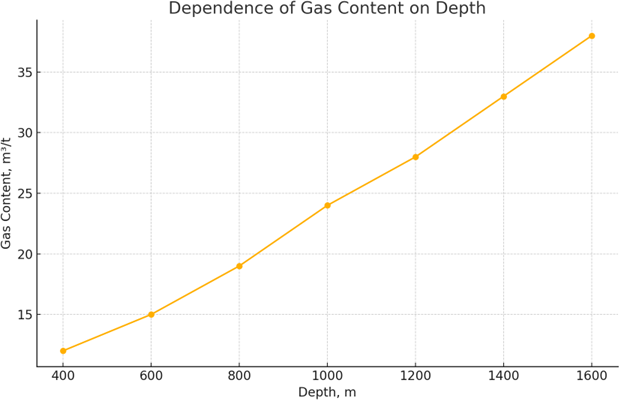
\includegraphics[width=\textwidth]{media/gorn2/image52}
		\caption*{Fig.1 - Dependence of Gas Content on Depth in Karaganda Basin}
	\end{subfigure}
	\begin{subfigure}{0.48\textwidth}
		\centering
		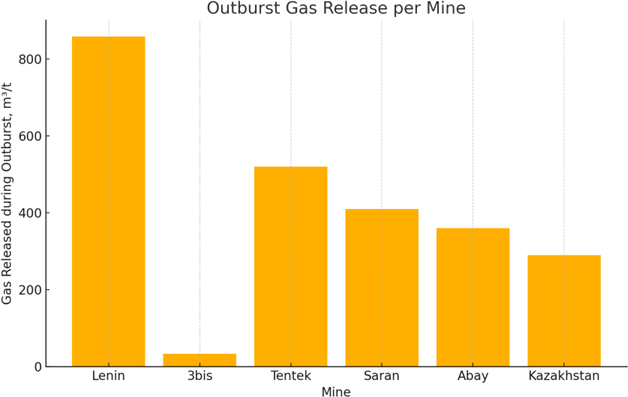
\includegraphics[width=\textwidth]{media/gorn2/image53}
		\caption*{Fig.2 - Outburst Gas Release per Mine in Karaganda Basin}
	\end{subfigure}
\end{figure}

\begin{multicols}{2}
We investigate possible options for reducing the outburst hazard by
influencing the parameters included in (3). A decrease in the
temperature of coal in the outburst-hazardous zone leads to an increase
in the threshold at which coal dispersion and gas release due to the
diffusion mechanism are possible (Table 2).
\end{multicols}

\tcap{Table 2 - Influence of coal temperature on the threshold stress ($\sigma_k$) for dispersion and gas release in the outburst - hazardous zone}
\begin{longtblr}[
  label = none,
  entry = none,
]{
  cells = {c},
  hlines,
  vlines,
}
{
Coal temperature, t\textsuperscript{о}С} & 20 & 15 & 10 & 5 & 0\\
$\sigma_k$, МPа & 30,5 & 41,0 & 51,50 & 62,1 & 72,6
\end{longtblr}

\begin{multicols}{2}
Reducing the temperature of coal by 5\textsuperscript{о}C leads to an
increase in strength by about 10 MPa. When degassing a coal seam, the
numerical values \emph{σ\textsubscript{k }}shown in Table 1 increase by
a factor of 1.30‑1.45.

{\bfseries Conclusion.} The mechanism of sudden outbursts and the causes of
their occurrence differ in the aggregate assessment of the participation
of gas in them, the stress-strain state of the massif, as well as the
physical, mechanical and physico-chemical properties of the intersected
massif along the front of the mining operation.

Results show that coal porosity and methane saturation are directly
correlated with the likelihood of sudden outbursts. Gas pressure at
depths above 500 m can exceed critical strength thresholds. Graphs in
Figure 1 and Figure 2 illustrate this dependence.

At the same time, coal-sorbed methane plays a significant role in the
implementation of a sudden outburst. With rapid stress relief in a
gas-saturated coal seam, especially near or in the zone of tectonic
disturbances characterized by the presence of disturbed coal bundles,
this gas disperses coal with simultaneous avalanche-like methane release
and removal of the destroyed rock mass in the bottom-hole part into the
mine.
\end{multicols}

\begin{center}
{\bfseries References}
\end{center}

\begin{references}
1. Katalog vnezapnykh vybrosov uglya i gaza, proisshedshikh na shakhtakh
Karagandinskogo basseina. - Karaganda: GU UD AO "ArselorMittal
Temirtau", 2018. - 171 s.{[}in Russian{]}

2. Tsai B.N., Shontayev A.D. Analiz vybrosov uglya i gaza, proisshedshikh
na shakhtakh Karagandinskogo basseina // Trudy Mezhdunarodnoi nauchnoi
konferentsii «Nauka i obrazovanie -- vedushchii faktor strategii
«Kazakhstan-2030». -- Karaganda, 2008. - S.87-90. {[}in Russian{]}

3. Tsai B.N., Bondarenko T.T., Shontayev A.D., Amurgalinov S.T.
Degazatsionnye skvazhiny i gidrorazryv plasta kak sposoby
predotvrashcheniya vnezapnykh vybrosov uglya i gaza // Materialy II
Mezhdunarodnoi nauchnoi konferentsii «Innovatsionnoe razvitie i
vostrebovannost'{} nauki v sovremennom KazakhstanE». --
Almaty, 2008. -- S.91-93. {[}in Russian{]}

4. Shontayev A.D., Dudich O.N. O mekhanizme vnezapnykh vybrosov uglya i
gaza // Materialy \\Mezhvuzovskoi studencheskoi nauchnoi konferentsii
«Student i nauchno-tekhnicheskii progress». -- \\Karaganda, 2009. -- S.
155-157. {[}in Russian{]}

5. Dokukin A.V., Airuni A.T., Ehttinger I.I.,
Bol' shinskii M.I., Zverev I.V., Dolgova M.O.
Bor' ba s vnezapnymi vybrosami uglya i gaza v shakhtakh /
Vestnik AN SSSR. - M.: 1984. --№ 12. - S.44‑45. {[}in Russian{]}

6. Zhekamukhov M.K., Zhekamukhova I.M. K probleme vnezapnykh vybrosov
uglya i gaza / Ehlektronnyi zhurnal «Issledovano v Rossii», 2003.-S.
526‑538. URL: \href{https://cyberleninka.ru/article/n/k-probleme-vnezapnyh-vybrosov-uglya-i-gaza-v-shahtah}{https://cyberleninka.ru} .- Дata
obrashhenija: \\02.02.2025. {[}in Russian{]}

7. Regel'{} V.R., Slutsker A.I., Tomashevskii Eh.K.
Kineticheskaya priroda prochnosti tverdykh tel. -- M.: Nauka, 1974. --
376 s.
DOI~\href{https://doi.org/10.3367/UFNr.0106.197202a.0193}{10.3367/UFNr.0106.197202a.0193}.
{[}in Russian{]}

8. Tsai B.N. Vliyanie teplovogo dvizheniya molekul na protsess
razrusheniya gornykh porod / Izv. vuzov. Gornyi zhurnal, 1982. -- № 10.
-- S.3-7. {[}in Russian{]}

9. Kucheryavyi F.I., Mikhalyuk A.V., Demchenko L.A. Ehnergiya aktivatsii
i ehnergoemkost'{} razrusheniya gornykh porod // Izv.
vuzov. Gornyi zhurnal, 1980. -- № 5. -- S.57-63. {[}in Russian{]}

10. \href{https://www.researchgate.net/scientific-contributions/Peng-Li-2180480712?_tp=eyJjb250ZXh0Ijp7ImZpcnN0UGFnZSI6InB1YmxpY2F0aW9uIiwicGFnZSI6InB1YmxpY2F0aW9uIn19}{Peng
Li},
\href{https://www.researchgate.net/scientific-contributions/Yaolin-Cao-2210424180?_tp=eyJjb250ZXh0Ijp7ImZpcnN0UGFnZSI6InB1YmxpY2F0aW9uIiwicGFnZSI6InB1YmxpY2F0aW9uIn19}{Yaolin
Cao} et al. Desorption Characterization of Methane in Coal with
Different Moisture Contents and Its Influence on Outburst Prediction//
Advances in Civil Engineering.-2021.-Vol.2.- P.1-10.
DOI:\href{http://dx.doi.org/10.1155/2021/6797786}{10.1155/2021/6797786}

11. Fatemeh~Soleimani,~Guangyao~Si,~Hamid~Roshan,~Zhenyu~Zhang.
Numerical modelling of coal and gas outburst initiation using energy
balance principles//Fuel.-2023.-Vol.334:126687 DOI\\
10.1016/j.fuel.2022.126687.

12. Liu, Q., Wang, Z., et al. (2018). Influence of coal strength and gas
pressure on outburst risk// Fuel, 223, 420--430.

13. \href{https://journals.sagepub.com/doi/10.1155/2023/5201794?icid=int.sj-full-text.similar-articles.4\#con1}{Ran~Wang},~\href{https://journals.sagepub.com/doi/10.1155/2023/5201794?icid=int.sj-full-text.similar-articles.4\#con2}{Xianbo~Su}
et al. Experimental Investigation of the Thermal Expansion
Characteristics of Coal Induced by Gas
Adsorption//\href{https://www.researchgate.net/journal/SSRN-Electronic-Journal-1556-5068}{SSRN
Electronic Journal}.-2022.-
\href{https://doi.org/\%20\%20\%20DOI\%2010.1155/2023/5201794}{DOI
10.1155/2023/5201794}

14. Drizhd N.A. Doklad na 6-om Mezhdunarodnom gorno-metallurgicheskom
Kongresse «Astana Mining \& Metallurgy» (AMM), 17 ijunja 2015 g.,
Astana. - 19 s.{[}in Russian{]}

15. Drizhd N.A., Sharipov N.H. O vozmozhnosti promyshlennoj dobychi
metana v Karagandinskom \\bassejne // Sekcija: Jenergetika. Materialy
konferencii «Social' noe izmerenie evrazijskoj
integracii». - Karaganda: KarGTU, 2016. {[}in Russian{]}
\end{references}

\begin{authorinfo}
\emph{{\bfseries Information about the authors}}

Shontayev A.D. - PhD, Associate Professor of Kazakh University of
Technology and Business, Astana, Kazakhstan, e-mail: \href{mailto:shon_oskar@mail.ru}{\nolinkurl{shon\_oskar@mail.ru}},

Demina T.V. - Сandidate of Technical Sciences, Associate Professor of
Ural State Mining University, Ekaterinburg, Russian Federation, 
e-mail: \href{mailto:baiz76@mail.ru}{fgz.bgp@m.ursmu.ru};

Shontaev D.S. - Сandidate of Technical Sciences, Associate Professor of
Kazakh University of Technology and Business, Astana, Kazakhstan, 
e-mail: \href{mailto:baiz76@mail.ru}{dshontaev@mail.ru};

Demin V.F. - Doctor of Technical Sciences, Professor of Saginov
Technical University, Karagandy, Kazakhstan, 
e-mail: \\\href{mailto:diana_meiram@mail.ru}{vladfdemin@mail.ru};

Meiram D. D. - Master, Doctoral student of Saginov Technical University,
Karagandy, Kazakhstan, e-mail: \\\href{mailto:diana_meiram@mail.ru}{\nolinkurl{diana\_meiram@mail.ru}},

\emph{{\bfseries Сведения об авторах}}

Шонтаев А.Д. - PhD, асс.профессор Казахского университета технологии и
бизнеса, Астана, Казахстан,
e-mail: \\\href{mailto:shon_oskar@mail.ru}{\nolinkurl{shon\_oskar@mail.ru}};

Демина Т.В. - к.т.н., доцент Уральского государственного горного
университета, Екатеринбург, Российская Федерация,  e-mail: \href{mailto:baiz76@mail.ru}{fgz.bgp@m.ursmu.ru};

Шонтаев Д.С. - к.т.н., асс.профессор Казахского университета технологии
и бизнеса, Астана, Казахстан, 
e-mail: \\\href{mailto:baiz76@mail.ru}{dshontaev@mail.ru};

Демин В.Ф. - д.т.н., профессор Карагандинского технического университета
имени А.Сагинова, Караганды, Казахстан, 
e-mail: \href{mailto:diana_meiram@mail.ru}{vladfdemin@mail.ru};

Мейрам Д.Д. - магистр, докторант Карагандинского технического
университета имени А.Сагинова, Караганды, Казахстан, 
e-mail: \href{mailto:diana_meiram@mail.ru}{\nolinkurl{diana\_meiram@mail.ru}}\
\end{authorinfo}
